\chapter{Caminos más cortos}

\index{camino más corto}

Encontrar un camino más corto entre dos nodos
de un grafo
es un problema importante que tiene muchas
aplicaciones prácticas.
Por ejemplo, un problema natural relacionado con una red de carreteras
es calcular la menor longitud posible de una ruta
entre dos ciudades, dadas las longitudes de las carreteras.

En un grafo no ponderado, la longitud de un camino es igual
al número de sus aristas, y podemos
simplemente usar la búsqueda en anchura para encontrar
un camino más corto.
Sin embargo, en este capítulo nos enfocamos en
grafos ponderados
donde se necesitan algoritmos más sofisticados
para encontrar caminos más cortos.

\section{Algoritmo de Bellman–Ford}

\index{algoritmo de Bellman–Ford}

El \key{algoritmo de Bellman–Ford}\footnote{El algoritmo lleva el nombre de
R. E. Bellman y L. R. Ford, quienes lo publicaron de forma independiente
en 1958 y 1956, respectivamente \cite{bel58,for56a}.} encuentra
caminos más cortos desde un nodo inicial a todos
los nodos del grafo.
El algoritmo puede procesar todo tipo de grafos,
siempre que el grafo no contenga un
ciclo de longitud negativa.
Si el grafo contiene un ciclo negativo,
el algoritmo puede detectarlo.

El algoritmo lleva un registro de las distancias
desde el nodo inicial a todos los nodos del grafo.
Inicialmente, la distancia al nodo inicial es 0
y la distancia a todos los demás nodos es infinita.
El algoritmo reduce las distancias encontrando
aristas que acortan los caminos hasta que no es
posible reducir ninguna distancia.

\subsubsection{Ejemplo}

Consideremos cómo funciona el algoritmo de Bellman–Ford
en el siguiente grafo:
\begin{center}
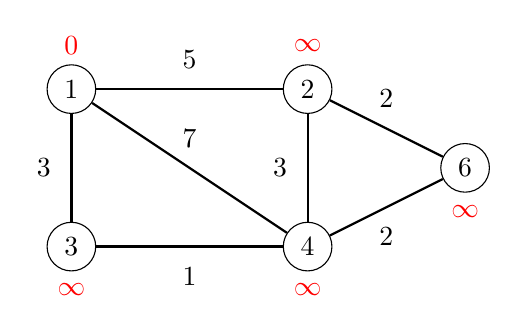
\begin{tikzpicture}
\node[draw, circle] (1) at (1,3) {1};
\node[draw, circle] (2) at (4,3) {2};
\node[draw, circle] (3) at (1,1) {3};
\node[draw, circle] (4) at (4,1) {4};
\node[draw, circle] (5) at (6,2) {6};
\node[color=red] at (1,3+0.55) {$0$};
\node[color=red] at (4,3+0.55) {$\infty$};
\node[color=red] at (1,1-0.55) {$\infty$};
\node[color=red] at (4,1-0.55) {$\infty$};
\node[color=red] at (6,2-0.55) {$\infty$};
\path[draw,thick,-] (1) -- node[font=\small,label=above:5] {} (2);
\path[draw,thick,-] (1) -- node[font=\small,label=left:3] {} (3);
\path[draw,thick,-] (3) -- node[font=\small,label=below:1] {} (4);
\path[draw,thick,-] (2) -- node[font=\small,label=left:3] {} (4);
\path[draw,thick,-] (2) -- node[font=\small,label=above:2] {} (5);
\path[draw,thick,-] (4) -- node[font=\small,label=below:2] {} (5);
\path[draw,thick,-] (1) -- node[font=\small,label=above:7] {} (4);
\end{tikzpicture}
\end{center}
A cada nodo del grafo se le asigna una distancia.
Inicialmente, la distancia al nodo inicial es 0,
y la distancia a todos los demás nodos es infinita.

El algoritmo busca aristas que reduzcan distancias.
Primero, todas las aristas desde el nodo 1 reducen distancias:
\begin{center}
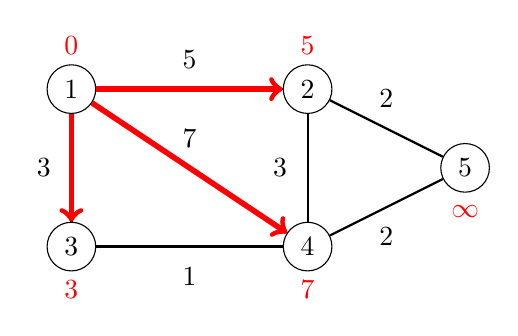
\begin{tikzpicture}
\node[draw, circle] (1) at (1,3) {1};
\node[draw, circle] (2) at (4,3) {2};
\node[draw, circle] (3) at (1,1) {3};
\node[draw, circle] (4) at (4,1) {4};
\node[draw, circle] (5) at (6,2) {5};
\node[color=red] at (1,3+0.55) {$0$};
\node[color=red] at (4,3+0.55) {$5$};
\node[color=red] at (1,1-0.55) {$3$};
\node[color=red] at (4,1-0.55) {$7$};
\node[color=red] at (6,2-0.55) {$\infty$};
\path[draw,thick,-] (1) -- node[font=\small,label=above:5] {} (2);
\path[draw,thick,-] (1) -- node[font=\small,label=left:3] {} (3);
\path[draw,thick,-] (3) -- node[font=\small,label=below:1] {} (4);
\path[draw,thick,-] (2) -- node[font=\small,label=left:3] {} (4);
\path[draw,thick,-] (2) -- node[font=\small,label=above:2] {} (5);
\path[draw,thick,-] (4) -- node[font=\small,label=below:2] {} (5);
\path[draw,thick,-] (1) -- node[font=\small,label=above:7] {} (4);

\path[draw=red,thick,->,line width=2pt] (1) -- (2);
\path[draw=red,thick,->,line width=2pt] (1) -- (3);
\path[draw=red,thick,->,line width=2pt] (1) -- (4);
\end{tikzpicture}
\end{center}
Después de esto, las aristas
$2 \rightarrow 5$ y $3 \rightarrow 4$
reducen distancias:
\begin{center}
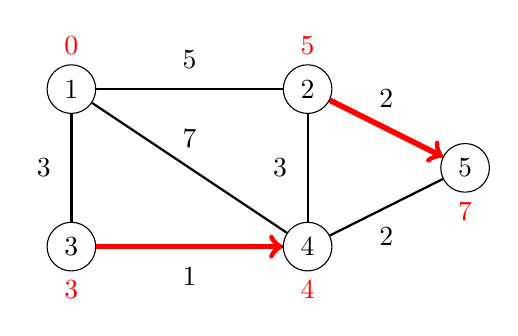
\begin{tikzpicture}
\node[draw, circle] (1) at (1,3) {1};
\node[draw, circle] (2) at (4,3) {2};
\node[draw, circle] (3) at (1,1) {3};
\node[draw, circle] (4) at (4,1) {4};
\node[draw, circle] (5) at (6,2) {5};
\node[color=red] at (1,3+0.55) {$0$};
\node[color=red] at (4,3+0.55) {$5$};
\node[color=red] at (1,1-0.55) {$3$};
\node[color=red] at (4,1-0.55) {$4$};
\node[color=red] at (6,2-0.55) {$7$};
\path[draw,thick,-] (1) -- node[font=\small,label=above:5] {} (2);
\path[draw,thick,-] (1) -- node[font=\small,label=left:3] {} (3);
\path[draw,thick,-] (3) -- node[font=\small,label=below:1] {} (4);
\path[draw,thick,-] (2) -- node[font=\small,label=left:3] {} (4);
\path[draw,thick,-] (2) -- node[font=\small,label=above:2] {} (5);
\path[draw,thick,-] (4) -- node[font=\small,label=below:2] {} (5);
\path[draw,thick,-] (1) -- node[font=\small,label=above:7] {} (4);

\path[draw=red,thick,->,line width=2pt] (2) -- (5);
\path[draw=red,thick,->,line width=2pt] (3) -- (4);
\end{tikzpicture}
\end{center}
Finalmente, hay un cambio más:
\begin{center}
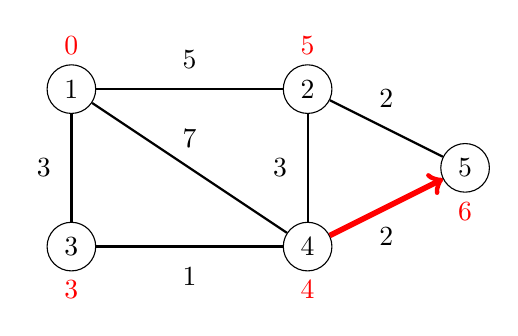
\begin{tikzpicture}
\node[draw, circle] (1) at (1,3) {1};
\node[draw, circle] (2) at (4,3) {2};
\node[draw, circle] (3) at (1,1) {3};
\node[draw, circle] (4) at (4,1) {4};
\node[draw, circle] (5) at (6,2) {5};
\node[color=red] at (1,3+0.55) {$0$};
\node[color=red] at (4,3+0.55) {$5$};
\node[color=red] at (1,1-0.55) {$3$};
\node[color=red] at (4,1-0.55) {$4$};
\node[color=red] at (6,2-0.55) {$6$};
\path[draw,thick,-] (1) -- node[font=\small,label=above:5] {} (2);
\path[draw,thick,-] (1) -- node[font=\small,label=left:3] {} (3);
\path[draw,thick,-] (3) -- node[font=\small,label=below:1] {} (4);
\path[draw,thick,-] (2) -- node[font=\small,label=left:3] {} (4);
\path[draw,thick,-] (2) -- node[font=\small,label=above:2] {} (5);
\path[draw,thick,-] (4) -- node[font=\small,label=below:2] {} (5);
\path[draw,thick,-] (1) -- node[font=\small,label=above:7] {} (4);

\path[draw=red,thick,->,line width=2pt] (4) -- (5);
\end{tikzpicture}
\end{center}

Después de esto, ninguna arista puede reducir ninguna distancia.
Esto significa que las distancias son definitivas,
y hemos calculado con éxito
las distancias más cortas
desde el nodo inicial a todos los nodos del grafo.

Por ejemplo, la distancia más corta 3
del nodo 1 al nodo 5 corresponde a
el siguiente camino:

\begin{center}
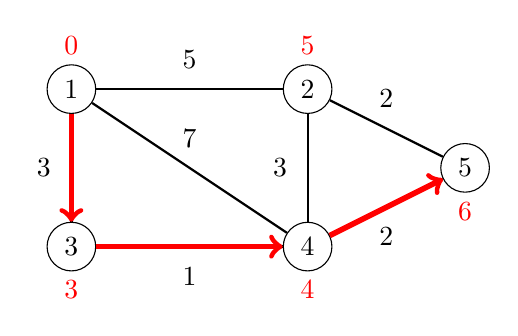
\begin{tikzpicture}
\node[draw, circle] (1) at (1,3) {1};
\node[draw, circle] (2) at (4,3) {2};
\node[draw, circle] (3) at (1,1) {3};
\node[draw, circle] (4) at (4,1) {4};
\node[draw, circle] (5) at (6,2) {5};
\node[color=red] at (1,3+0.55) {$0$};
\node[color=red] at (4,3+0.55) {$5$};
\node[color=red] at (1,1-0.55) {$3$};
\node[color=red] at (4,1-0.55) {$4$};
\node[color=red] at (6,2-0.55) {$6$};
\path[draw,thick,-] (1) -- node[font=\small,label=above:5] {} (2);
\path[draw,thick,-] (1) -- node[font=\small,label=left:3] {} (3);
\path[draw,thick,-] (3) -- node[font=\small,label=below:1] {} (4);
\path[draw,thick,-] (2) -- node[font=\small,label=left:3] {} (4);
\path[draw,thick,-] (2) -- node[font=\small,label=above:2] {} (5);
\path[draw,thick,-] (4) -- node[font=\small,label=below:2] {} (5);
\path[draw,thick,-] (1) -- node[font=\small,label=above:7] {} (4);

\path[draw=red,thick,->,line width=2pt] (1) -- (3);
\path[draw=red,thick,->,line width=2pt] (3) -- (4);
\path[draw=red,thick,->,line width=2pt] (4) -- (5);
\end{tikzpicture}
\end{center}

\subsubsection{Implementación}

La siguiente implementación del
algoritmo de Bellman–Ford determina las distancias más cortas
desde un nodo $x$ a todos los nodos del grafo.
El código supone que el grafo está almacenado
como una lista de aristas \texttt{edges}
que consiste en tuplas de la forma $(a,b,w)$,
lo que significa que hay una arista del nodo $a$ al nodo $b$
con peso $w$.

El algoritmo consiste en $n-1$ rondas,
y en cada ronda el algoritmo recorre
todas las aristas del grafo e intenta
reducir las distancias.
El algoritmo construye un arreglo \texttt{distance}
que contendrá las distancias desde $x$
a todos los nodos del grafo.
La constante \texttt{INF} denota una distancia infinita.

\begin{lstlisting}
for (int i = 1; i <= n; i++) distance[i] = INF;
distance[x] = 0;
for (int i = 1; i <= n-1; i++) {
    for (auto e : edges) {
        int a, b, w;
        tie(a, b, w) = e;
        distance[b] = min(distance[b], distance[a]+w);
    }
}
\end{lstlisting}

La complejidad temporal del algoritmo es $O(nm)$,
porque el algoritmo consiste en $n-1$ rondas y
recorre todas las $m$ aristas durante una ronda.
Si no hay ciclos negativos en el grafo,
todas las distancias son definitivas después de $n-1$ rondas,
porque cada camino más corto puede contener a lo sumo $n-1$ aristas.

En la práctica, las distancias definitivas usualmente
se pueden encontrar más rápido que en $n-1$ rondas.
Así, una forma posible de hacer el algoritmo más eficiente
es detener el algoritmo si ninguna distancia
se puede reducir durante una ronda.

\subsubsection{Ciclos negativos}

\index{ciclo negativo}

El algoritmo de Bellman–Ford también se puede usar para
comprobar si el grafo contiene un ciclo de longitud negativa.
Por ejemplo, el grafo

\begin{center}
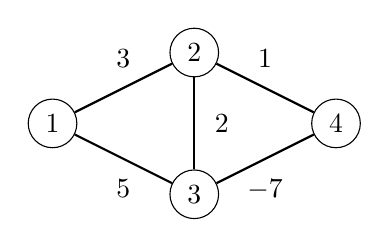
\begin{tikzpicture}[scale=0.9]
\node[draw, circle] (1) at (0,0) {$1$};
\node[draw, circle] (2) at (2,1) {$2$};
\node[draw, circle] (3) at (2,-1) {$3$};
\node[draw, circle] (4) at (4,0) {$4$};

\path[draw,thick,-] (1) -- node[font=\small,label=above:$3$] {} (2);
\path[draw,thick,-] (2) -- node[font=\small,label=above:$1$] {} (4);
\path[draw,thick,-] (1) -- node[font=\small,label=below:$5$] {} (3);
\path[draw,thick,-] (3) -- node[font=\small,label=below:$-7$] {} (4);
\path[draw,thick,-] (2) -- node[font=\small,label=right:$2$] {} (3);
\end{tikzpicture}
\end{center}
\noindent
contiene un ciclo negativo
$2 \rightarrow 3 \rightarrow 4 \rightarrow 2$
de longitud $-4$.

Si el grafo contiene un ciclo negativo,
podemos acortar infinitas veces
cualquier camino que contenga el ciclo repitiendo el ciclo
una y otra vez.
Así, el concepto de camino más corto
no tiene sentido en esta situación.

Un ciclo negativo se puede detectar
usando el algoritmo de Bellman–Ford
ejecutando el algoritmo durante $n$ rondas.
Si la última ronda reduce alguna distancia,
el grafo contiene un ciclo negativo.
Nótese que este algoritmo se puede usar para
buscar
un ciclo negativo en todo el grafo
independientemente del nodo inicial.

\subsubsection{Algoritmo SPFA}

\index{algoritmo SPFA}

El \key{algoritmo SPFA} (''Shortest Path Faster Algorithm'') \cite{fan94}
es una variante del algoritmo de Bellman–Ford,
que a menudo es más eficiente que el algoritmo original.
El algoritmo SPFA no recorre todas las aristas en cada ronda,
sino que, en su lugar, elige las aristas a examinar
de una forma más inteligente.

El algoritmo mantiene una cola de nodos que podrían
usarse para reducir las distancias.
Primero, el algoritmo añade el nodo inicial $x$
a la cola.
Luego, el algoritmo siempre procesa el
primer nodo de la cola, y cuando una arista
$a \rightarrow b$ reduce una distancia,
el nodo $b$ se añade a la cola.
%
% The following implementation uses a
% \texttt{queue} \texttt{q}.
% In addition, an array \texttt{inqueue} indicates
% if a node is already in the queue,
% in which case the algorithm does not add
% the node to the queue again.
%
% \begin{lstlisting}
% for (int i = 1; i <= n; i++) distance[i] = INF;
% distance[x] = 0;
% q.push(x);
% while (!q.empty()) {
%     int a = q.front(); q.pop();
%     inqueue[a] = false;
%     for (auto b : v[a]) {
%         if (distance[a]+b.second < distance[b.first]) {
%             distance[b.first] = distance[a]+b.second;
%             if (!inqueue[b]) {q.push(b); inqueue[b] = true;}
%         }
%     }
% }
% \end{lstlisting}

La eficiencia del algoritmo SPFA depende
de la estructura del grafo:
el algoritmo a menudo es eficiente,
pero su complejidad temporal en el peor caso sigue siendo
$O(nm)$ y es posible crear entradas
que hagan el algoritmo tan lento como el
algoritmo de Bellman–Ford original.

\section{Algoritmo de Dijkstra}

\index{algoritmo de Dijkstra}

El \key{algoritmo de Dijkstra}\footnote{E. W. Dijkstra publicó el algoritmo en 1959 \cite{dij59};
sin embargo, su artículo original no menciona cómo implementar el algoritmo eficientemente.}
encuentra caminos
más cortos desde el nodo inicial a todos los nodos del grafo,
como el algoritmo de Bellman–Ford.
El beneficio del algoritmo de Dijkstra es que
es más eficiente y se puede usar para
procesar grafos grandes.
Sin embargo, el algoritmo requiere que no
haya aristas de peso negativo en el grafo.

Como el algoritmo de Bellman–Ford,
el algoritmo de Dijkstra mantiene distancias
a los nodos y las reduce durante la búsqueda.
El algoritmo de Dijkstra es eficiente, porque
solo procesa
cada arista del grafo una vez, usando el hecho
de que no hay aristas negativas.

\subsubsection{Ejemplo}

Consideremos cómo funciona el algoritmo de Dijkstra
en el siguiente grafo cuando el
nodo inicial es el nodo 1:
\begin{center}
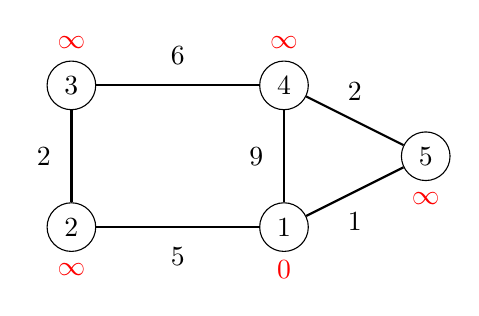
\begin{tikzpicture}[scale=0.9]
\node[draw, circle] (1) at (1,3) {3};
\node[draw, circle] (2) at (4,3) {4};
\node[draw, circle] (3) at (1,1) {2};
\node[draw, circle] (4) at (4,1) {1};
\node[draw, circle] (5) at (6,2) {5};

\node[color=red] at (1,3+0.6) {$\infty$};
\node[color=red] at (4,3+0.6) {$\infty$};
\node[color=red] at (1,1-0.6) {$\infty$};
\node[color=red] at (4,1-0.6) {$0$};
\node[color=red] at (6,2-0.6) {$\infty$};

\path[draw,thick,-] (1) -- node[font=\small,label=above:6] {} (2);
\path[draw,thick,-] (1) -- node[font=\small,label=left:2] {} (3);
\path[draw,thick,-] (3) -- node[font=\small,label=below:5] {} (4);
\path[draw,thick,-] (2) -- node[font=\small,label=left:9] {} (4);
\path[draw,thick,-] (2) -- node[font=\small,label=above:2] {} (5);
\path[draw,thick,-] (4) -- node[font=\small,label=below:1] {} (5);
\end{tikzpicture}
\end{center}
Como en el algoritmo de Bellman–Ford,
inicialmente la distancia al nodo inicial es 0
y la distancia a todos los demás nodos es infinita.

En cada paso, el algoritmo de Dijkstra selecciona un nodo
que todavía no ha sido procesado y cuya distancia
sea lo más pequeña posible.
El primer nodo de este tipo es el nodo 1 con distancia 0.

Cuando se selecciona un nodo, el algoritmo
recorre todas las aristas que empiezan en el nodo
y reduce las distancias usándolas:
\begin{center}
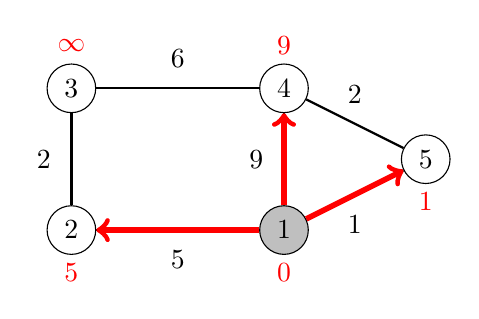
\begin{tikzpicture}[scale=0.9]
\node[draw, circle] (1) at (1,3) {3};
\node[draw, circle] (2) at (4,3) {4};
\node[draw, circle] (3) at (1,1) {2};
\node[draw, circle, fill=lightgray] (4) at (4,1) {1};
\node[draw, circle] (5) at (6,2) {5};

\node[color=red] at (1,3+0.6) {$\infty$};
\node[color=red] at (4,3+0.6) {$9$};
\node[color=red] at (1,1-0.6) {$5$};
\node[color=red] at (4,1-0.6) {$0$};
\node[color=red] at (6,2-0.6) {$1$};

\path[draw,thick,-] (1) -- node[font=\small,label=above:6] {} (2);
\path[draw,thick,-] (1) -- node[font=\small,label=left:2] {} (3);
\path[draw,thick,-] (3) -- node[font=\small,label=below:5] {} (4);
\path[draw,thick,-] (2) -- node[font=\small,label=left:9] {} (4);
\path[draw,thick,-] (2) -- node[font=\small,label=above:2] {} (5);
\path[draw,thick,-] (4) -- node[font=\small,label=below:1] {} (5);

\path[draw=red,thick,->,line width=2pt] (4) -- (2);
\path[draw=red,thick,->,line width=2pt] (4) -- (3);
\path[draw=red,thick,->,line width=2pt] (4) -- (5);
\end{tikzpicture}
\end{center}
En este caso,
las aristas desde el nodo 1 redujeron las distancias de
los nodos 2, 4 y 5, cuyas distancias ahora son 5, 9 y 1.

El siguiente nodo a procesar es el nodo 5 con distancia 1.
Esto reduce la distancia al nodo 4 de 9 a 3:
\begin{center}
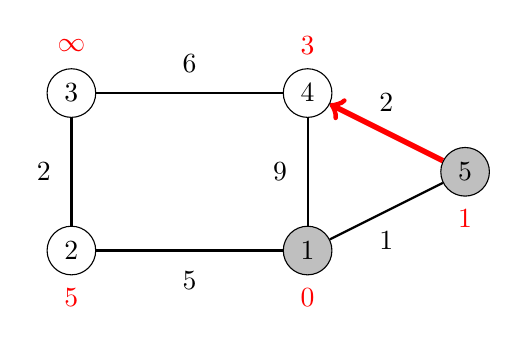
\begin{tikzpicture}
\node[draw, circle] (1) at (1,3) {3};
\node[draw, circle] (2) at (4,3) {4};
\node[draw, circle] (3) at (1,1) {2};
\node[draw, circle, fill=lightgray] (4) at (4,1) {1};
\node[draw, circle, fill=lightgray] (5) at (6,2) {5};

\node[color=red] at (1,3+0.6) {$\infty$};
\node[color=red] at (4,3+0.6) {$3$};
\node[color=red] at (1,1-0.6) {$5$};
\node[color=red] at (4,1-0.6) {$0$};
\node[color=red] at (6,2-0.6) {$1$};

\path[draw,thick,-] (1) -- node[font=\small,label=above:6] {} (2);
\path[draw,thick,-] (1) -- node[font=\small,label=left:2] {} (3);
\path[draw,thick,-] (3) -- node[font=\small,label=below:5] {} (4);
\path[draw,thick,-] (2) -- node[font=\small,label=left:9] {} (4);
\path[draw,thick,-] (2) -- node[font=\small,label=above:2] {} (5);
\path[draw,thick,-] (4) -- node[font=\small,label=below:1] {} (5);

\path[draw=red,thick,->,line width=2pt] (5) -- (2);
\end{tikzpicture}
\end{center}
Después de esto, el siguiente nodo es el nodo 4, que reduce
la distancia al nodo 3 a 9:
\begin{center}
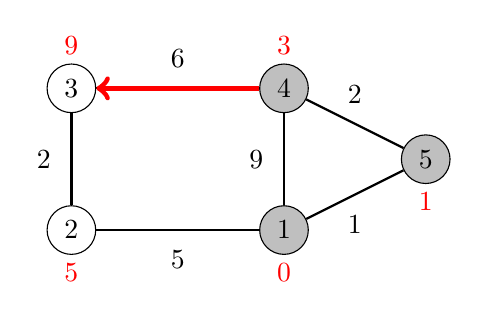
\begin{tikzpicture}[scale=0.9]
\node[draw, circle] (1) at (1,3) {3};
\node[draw, circle, fill=lightgray] (2) at (4,3) {4};
\node[draw, circle] (3) at (1,1) {2};
\node[draw, circle, fill=lightgray] (4) at (4,1) {1};
\node[draw, circle, fill=lightgray] (5) at (6,2) {5};

\node[color=red] at (1,3+0.6) {$9$};
\node[color=red] at (4,3+0.6) {$3$};
\node[color=red] at (1,1-0.6) {$5$};
\node[color=red] at (4,1-0.6) {$0$};
\node[color=red] at (6,2-0.6) {$1$};

\path[draw,thick,-] (1) -- node[font=\small,label=above:6] {} (2);
\path[draw,thick,-] (1) -- node[font=\small,label=left:2] {} (3);
\path[draw,thick,-] (3) -- node[font=\small,label=below:5] {} (4);
\path[draw,thick,-] (2) -- node[font=\small,label=left:9] {} (4);
\path[draw,thick,-] (2) -- node[font=\small,label=above:2] {} (5);
\path[draw,thick,-] (4) -- node[font=\small,label=below:1] {} (5);

\path[draw=red,thick,->,line width=2pt] (2) -- (1);
\end{tikzpicture}
\end{center}

Una propiedad notable del algoritmo de Dijkstra es que
siempre que se selecciona un nodo, su distancia es definitiva.
Por ejemplo, en este punto del algoritmo,
las distancias 0, 1 y 3 son las distancias definitivas
a los nodos 1, 5 y 4.

Después de esto, el algoritmo procesa los dos
nodos restantes, y las distancias definitivas son las siguientes:

\begin{center}
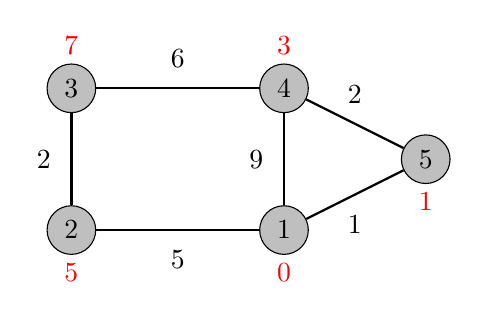
\begin{tikzpicture}[scale=0.9]
\node[draw, circle, fill=lightgray] (1) at (1,3) {3};
\node[draw, circle, fill=lightgray] (2) at (4,3) {4};
\node[draw, circle, fill=lightgray] (3) at (1,1) {2};
\node[draw, circle, fill=lightgray] (4) at (4,1) {1};
\node[draw, circle, fill=lightgray] (5) at (6,2) {5};

\node[color=red] at (1,3+0.6) {$7$};
\node[color=red] at (4,3+0.6) {$3$};
\node[color=red] at (1,1-0.6) {$5$};
\node[color=red] at (4,1-0.6) {$0$};
\node[color=red] at (6,2-0.6) {$1$};

\path[draw,thick,-] (1) -- node[font=\small,label=above:6] {} (2);
\path[draw,thick,-] (1) -- node[font=\small,label=left:2] {} (3);
\path[draw,thick,-] (3) -- node[font=\small,label=below:5] {} (4);
\path[draw,thick,-] (2) -- node[font=\small,label=left:9] {} (4);
\path[draw,thick,-] (2) -- node[font=\small,label=above:2] {} (5);
\path[draw,thick,-] (4) -- node[font=\small,label=below:1] {} (5);
\end{tikzpicture}
\end{center}

\subsubsection{Aristas negativas}

La eficiencia del algoritmo de Dijkstra se
basa en el hecho de que el grafo no
contiene aristas negativas.
Si hay una arista negativa,
el algoritmo puede dar resultados incorrectos.
Como ejemplo, considérese el siguiente grafo:

\begin{center}
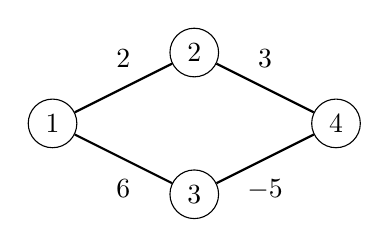
\begin{tikzpicture}[scale=0.9]
\node[draw, circle] (1) at (0,0) {$1$};
\node[draw, circle] (2) at (2,1) {$2$};
\node[draw, circle] (3) at (2,-1) {$3$};
\node[draw, circle] (4) at (4,0) {$4$};

\path[draw,thick,-] (1) -- node[font=\small,label=above:2] {} (2);
\path[draw,thick,-] (2) -- node[font=\small,label=above:3] {} (4);
\path[draw,thick,-] (1) -- node[font=\small,label=below:6] {} (3);
\path[draw,thick,-] (3) -- node[font=\small,label=below:$-5$] {} (4);
\end{tikzpicture}
\end{center}
\noindent
El camino más corto del nodo 1 al nodo 4 es
$1 \rightarrow 3 \rightarrow 4$
y su longitud es 1.
Sin embargo, el algoritmo de Dijkstra
encuentra el camino $1 \rightarrow 2 \rightarrow 4$
siguiendo las aristas de peso mínimo.
El algoritmo no tiene en cuenta que
en el otro camino, el peso $-5$
compensa el peso grande anterior $6$.

\subsubsection{Implementación}

La siguiente implementación del algoritmo de Dijkstra
calcula las distancias mínimas desde un nodo $x$
a los demás nodos del grafo.
El grafo está almacenado como listas de adyacencia
de manera que \texttt{adj[$a$]} contiene un par $(b,w)$
siempre que hay una arista del nodo $a$ al nodo $b$
con peso $w$.

Una implementación eficiente del algoritmo de Dijkstra
requiere que sea posible encontrar eficientemente el
nodo de distancia mínima que no ha sido procesado.
Una estructura de datos apropiada para esto es una cola de prioridad
que contiene los nodos ordenados por sus distancias.
Usando una cola de prioridad, el siguiente nodo a procesar
se puede recuperar en tiempo logarítmico.

En el siguiente código, la cola de prioridad
\texttt{q} contiene pares de la forma $(-d,x)$,
lo que significa que la distancia actual al nodo $x$ es $d$.
El arreglo $\texttt{distance}$ contiene la distancia a
cada nodo, y el arreglo $\texttt{processed}$ indica
si un nodo ha sido procesado.
Inicialmente la distancia es $0$ a $x$ e $\infty$ a todos los demás nodos.

\begin{lstlisting}
for (int i = 1; i <= n; i++) distance[i] = INF;
distance[x] = 0;
q.push({0,x});
while (!q.empty()) {
    int a = q.top().second; q.pop();
    if (processed[a]) continue;
    processed[a] = true;
    for (auto u : adj[a]) {
        int b = u.first, w = u.second;
        if (distance[a]+w < distance[b]) {
            distance[b] = distance[a]+w;
            q.push({-distance[b],b});
        }
    }
}
\end{lstlisting}

Nótese que la cola de prioridad contiene distancias
\emph{negativas} a los nodos.
La razón de esto es que la
versión por defecto de la cola de prioridad de C++ encuentra los elementos
máximos, mientras que nosotros queremos encontrar los elementos mínimos.
Al usar distancias negativas,
podemos usar directamente la cola de prioridad por defecto\footnote{Por
supuesto, también podríamos declarar la cola de prioridad como en el Capítulo 4.5
y usar distancias positivas, pero la implementación sería un poco más larga.}.
Nótese también que puede haber varias instancias del mismo
nodo en la cola de prioridad; sin embargo, solo la instancia con la
distancia mínima será procesada.

La complejidad temporal de la implementación anterior es
$O(n+m \log m)$, porque el algoritmo recorre
todos los nodos del grafo y añade por cada arista
a lo sumo una distancia a la cola de prioridad.

\section{Algoritmo de Floyd–Warshall}

\index{algoritmo de Floyd–Warshall}

El \key{algoritmo de Floyd–Warshall}\footnote{El algoritmo
lleva el nombre de R. W. Floyd y S. Warshall,
quienes lo publicaron de forma independiente en 1962 \cite{flo62,war62}.}
proporciona una forma alternativa de abordar el problema
de encontrar caminos más cortos.
A diferencia de los otros algoritmos de este capítulo,
encuentra todos los caminos más cortos entre los nodos
en una sola ejecución.

El algoritmo mantiene un arreglo bidimensional
que contiene las distancias entre los nodos.
Primero, las distancias se calculan usando solo
aristas directas entre los nodos,
y después de esto, el algoritmo reduce las distancias
usando nodos intermedios en los caminos.

\subsubsection{Ejemplo}

Consideremos cómo funciona el algoritmo de Floyd–Warshall
en el siguiente grafo:

\begin{center}
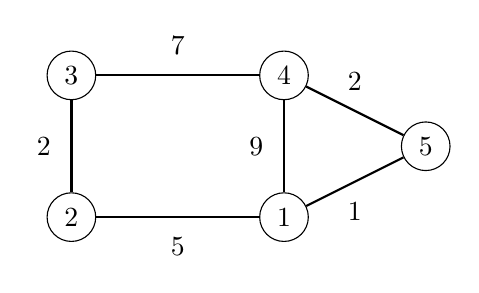
\begin{tikzpicture}[scale=0.9]
\node[draw, circle] (1) at (1,3) {$3$};
\node[draw, circle] (2) at (4,3) {$4$};
\node[draw, circle] (3) at (1,1) {$2$};
\node[draw, circle] (4) at (4,1) {$1$};
\node[draw, circle] (5) at (6,2) {$5$};

\path[draw,thick,-] (1) -- node[font=\small,label=above:7] {} (2);
\path[draw,thick,-] (1) -- node[font=\small,label=left:2] {} (3);
\path[draw,thick,-] (3) -- node[font=\small,label=below:5] {} (4);
\path[draw,thick,-] (2) -- node[font=\small,label=left:9] {} (4);
\path[draw,thick,-] (2) -- node[font=\small,label=above:2] {} (5);
\path[draw,thick,-] (4) -- node[font=\small,label=below:1] {} (5);
\end{tikzpicture}
\end{center}

Inicialmente, la distancia de cada nodo a sí mismo es $0$,
y la distancia entre los nodos $a$ y $b$ es $x$
si hay una arista entre los nodos $a$ y $b$ con peso $x$.
Todas las demás distancias son infinitas.

En este grafo, el arreglo inicial es el siguiente:
\begin{center}
\begin{tabular}{r|rrrrr}
 & 1 & 2 & 3 & 4 & 5 \\
\hline
1 & 0 & 5 & $\infty$ & 9 & 1 \\
2 & 5 & 0 & 2 & $\infty$ & $\infty$ \\
3 & $\infty$ & 2 & 0 & 7 & $\infty$ \\
4 & 9 & $\infty$ & 7 & 0 & 2 \\
5 & 1 & $\infty$ & $\infty$ & 2 & 0 \\
\end{tabular}
\end{center}
\vspace{10pt}
El algoritmo consiste en rondas consecutivas.
En cada ronda, el algoritmo selecciona un nuevo nodo
que puede actuar como nodo intermedio en los caminos de ahí en adelante,
y las distancias se reducen usando este nodo.

En la primera ronda, el nodo 1 es el nuevo nodo intermedio.
Hay un nuevo camino entre los nodos 2 y 4
de longitud 14, porque el nodo 1 los conecta.
También hay un nuevo camino
entre los nodos 2 y 5 de longitud 6.

\begin{center}
\begin{tabular}{r|rrrrr}
 & 1 & 2 & 3 & 4 & 5 \\
\hline
1 & 0 & 5 & $\infty$ & 9 & 1 \\
2 & 5 & 0 & 2 & \textbf{14} & \textbf{6} \\
3 & $\infty$ & 2 & 0 & 7 & $\infty$ \\
4 & 9 & \textbf{14} & 7 & 0 & 2 \\
5 & 1 & \textbf{6} & $\infty$ & 2 & 0 \\
\end{tabular}
\end{center}
\vspace{10pt}

En la segunda ronda, el nodo 2 es el nuevo nodo intermedio.
Esto crea nuevos caminos entre los nodos 1 y 3
y entre los nodos 3 y 5:

\begin{center}
\begin{tabular}{r|rrrrr}
 & 1 & 2 & 3 & 4 & 5 \\
\hline
1 & 0 & 5 & \textbf{7} & 9 & 1 \\
2 & 5 & 0 & 2 & 14 & 6 \\
3 & \textbf{7} & 2 & 0 & 7 & \textbf{8} \\
4 & 9 & 14 & 7 & 0 & 2 \\
5 & 1 & 6 & \textbf{8} & 2 & 0 \\
\end{tabular}
\end{center}
\vspace{10pt}

En la tercera ronda, el nodo 3 es el nuevo nodo intermedio.
Hay un nuevo camino entre los nodos 2 y 4:

\begin{center}
\begin{tabular}{r|rrrrr}
 & 1 & 2 & 3 & 4 & 5 \\
\hline
1 & 0 & 5 & 7 & 9 & 1 \\
2 & 5 & 0 & 2 & \textbf{9} & 6 \\
3 & 7 & 2 & 0 & 7 & 8 \\
4 & 9 & \textbf{9} & 7 & 0 & 2 \\
5 & 1 & 6 & 8 & 2 & 0 \\
\end{tabular}
\end{center}
\vspace{10pt}

El algoritmo continúa de esta manera,
hasta que todos los nodos han sido designados como nodos intermedios.
Después de que el algoritmo ha terminado, el arreglo contiene
las distancias mínimas entre cualesquiera dos nodos:

\begin{center}
\begin{tabular}{r|rrrrr}
 & 1 & 2 & 3 & 4 & 5 \\
\hline
1 & 0 & 5 & 7 & 3 & 1 \\
2 & 5 & 0 & 2 & 8 & 6 \\
3 & 7 & 2 & 0 & 7 & 8 \\
4 & 3 & 8 & 7 & 0 & 2 \\
5 & 1 & 6 & 8 & 2 & 0 \\
\end{tabular}
\end{center}

Por ejemplo, el arreglo nos dice que la
distancia más corta entre los nodos 2 y 4 es 8.
Esto corresponde al siguiente camino:

\begin{center}
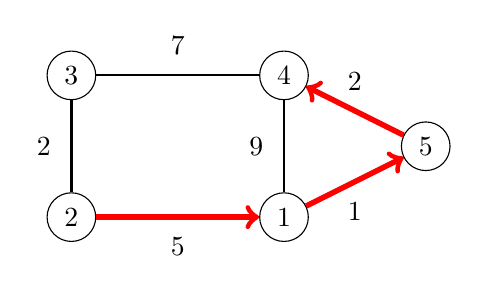
\begin{tikzpicture}[scale=0.9]
\node[draw, circle] (1) at (1,3) {$3$};
\node[draw, circle] (2) at (4,3) {$4$};
\node[draw, circle] (3) at (1,1) {$2$};
\node[draw, circle] (4) at (4,1) {$1$};
\node[draw, circle] (5) at (6,2) {$5$};

\path[draw,thick,-] (1) -- node[font=\small,label=above:7] {} (2);
\path[draw,thick,-] (1) -- node[font=\small,label=left:2] {} (3);
\path[draw,thick,-] (3) -- node[font=\small,label=below:5] {} (4);
\path[draw,thick,-] (2) -- node[font=\small,label=left:9] {} (4);
\path[draw,thick,-] (2) -- node[font=\small,label=above:2] {} (5);
\path[draw,thick,-] (4) -- node[font=\small,label=below:1] {} (5);

\path[draw=red,thick,->,line width=2pt] (3) -- (4);
\path[draw=red,thick,->,line width=2pt] (4) -- (5);
\path[draw=red,thick,->,line width=2pt] (5) -- (2);
\end{tikzpicture}
\end{center}

\subsubsection{Implementación}

La ventaja del
algoritmo de Floyd–Warshall es que es
fácil de implementar.
El siguiente código construye una
matriz de distancias donde $\texttt{distance}[a][b]$
es la distancia más corta entre los nodos $a$ y $b$.
Primero, el algoritmo inicializa \texttt{distance}
usando la matriz de adyacencia \texttt{adj} del grafo:

\begin{lstlisting}
for (int i = 1; i <= n; i++) {
    for (int j = 1; j <= n; j++) {
        if (i == j) distance[i][j] = 0;
        else if (adj[i][j]) distance[i][j] = adj[i][j];
        else distance[i][j] = INF;
    }
}
\end{lstlisting}
Después de esto, las distancias más cortas se pueden encontrar como sigue:
\begin{lstlisting}
for (int k = 1; k <= n; k++) {
    for (int i = 1; i <= n; i++) {
        for (int j = 1; j <= n; j++) {
            distance[i][j] = min(distance[i][j],
                                   distance[i][k]+distance[k][j]);
        }
    }
}
\end{lstlisting}

La complejidad temporal del algoritmo es $O(n^3)$,
porque contiene tres bucles anidados
que recorren los nodos del grafo.

Como la implementación del algoritmo de Floyd–Warshall
es simple, el algoritmo puede ser
una buena elección incluso si solo es necesario encontrar un
único camino más corto en el grafo.
Sin embargo, el algoritmo solo se puede usar cuando el grafo
es tan pequeño que una complejidad temporal cúbica es lo suficientemente rápida.
